\newpage
\section{课后习题:转动动力学}
\begin{example}[{\small Determine the Moment of Inertia of an Irregularly Shaped Object}---\refleaftext{solution3.1}]
	This problem describes one experimental method of
	determining the moment of inertia of an irregularly
	shaped object such as the \itr{payload}{有效负载} for a satellite. 
	\begin{center}
		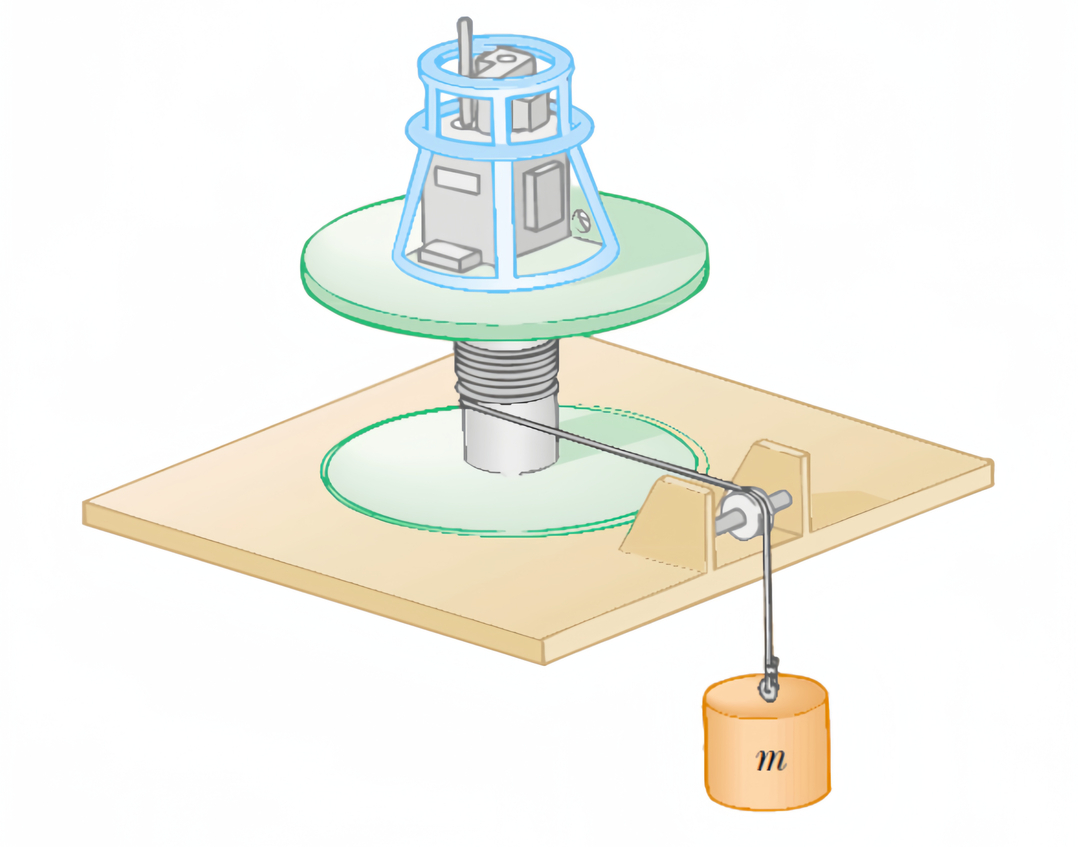
\includegraphics[width=0.6\textwidth]{chapter3_example_1}
	\end{center}
	
	The figure shows a mass $m$ \itr{suspended}{悬挂} by a \itr{cord}{绳子} \itr{wound}{被缠绕}
	around a spool of radius $r$, forming part of a \itr{turntable}{转台}
	supporting the object. When the mass is released from
	rest, it \itr{descends}{下降} through a distance $h$, acquiring a speed
	$\vec{v}$. Show that the moment of inertia $I$ of the equipment
	(including the turntable) is\quad$mr^2(\dfrac{2gh}{v^2}-1)$. 
\end{example}
%\refleaf*{solution3.1}[-75ex]
\begin{example}[Rolling Items---\refleaftext{solution3.2}]
	Three objects of \itr{uniform density}{均匀的密度} --- a \itr{solid sphere}{实心球}, a \itr{solid
	cylinder}{实心圆柱}, and a \itr{hollow cylinder}{空心圆柱} --- are placed at the top of
	an \itr{incline}{斜坡}. 
	\begin{center}
		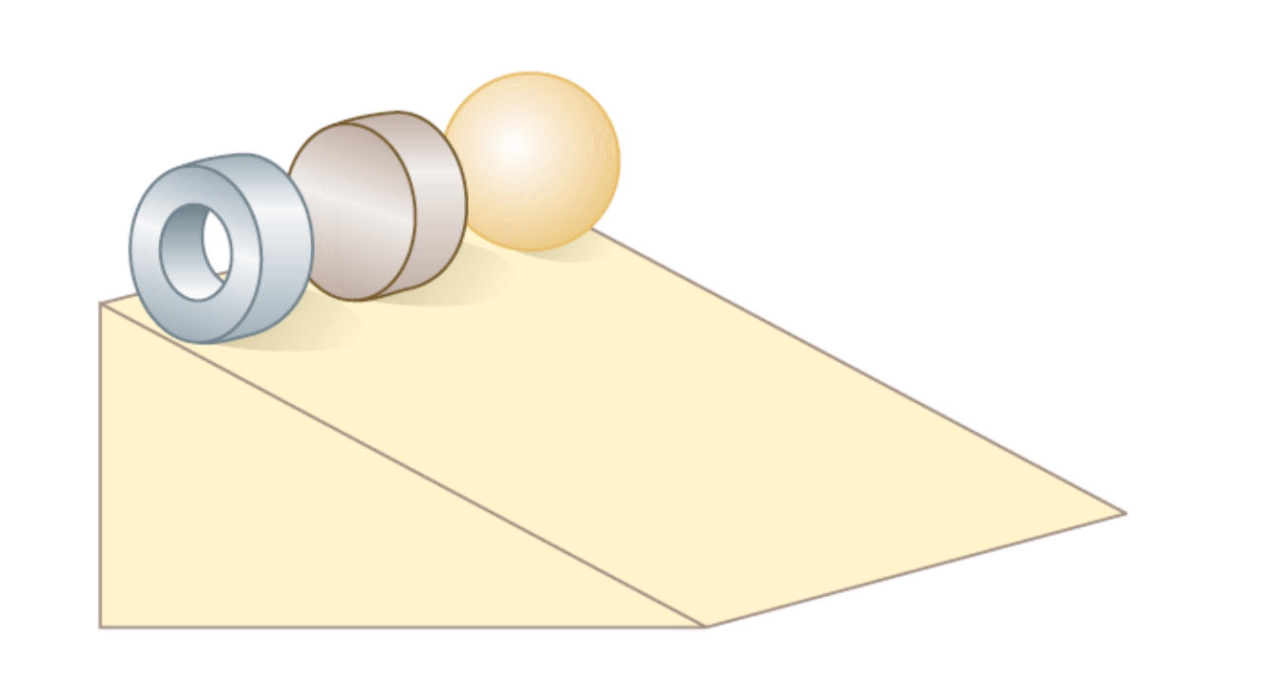
\includegraphics[width=0.6\textwidth]{chapter3_example_2}
	\end{center}
	If they all are released from rest
	at the same \itr{elevation}{高度} and roll without \itr{slipping}{滑动}, which object reaches the bottom first?
\end{example}
%\refleaf*{solution3.2}[-20ex]
\begin{example}[Calculation of the Moment of Inertia---\refleaftext{solution3.3}]
	A rod's \itr{linear density}{线密度} is given by $\lambda=kx$, where $x$ represents the distance from the point to the rod's center. 
	\ctikzfig{chapter3_example_3_3}
	Given the length of the rod $l$, try to calculate the moment of inertia of the rod, given the rotation axis at:
	
	(1) Center $O$ as the $y$ axis shows.
	
	(2) One end as the $y'$ axis shows.
\end{example}
\begin{example}[Massive \itr{Pulley}{滑轮}---\refleaftext{solution3.4}]
	Consider two \itr{cylinders}{圆柱} having masses $m_1$
	and $m_2$, where $m_1 < m_2$, connected by a
	string passing over a pulley. The pulley
	has a radius $R$ and moment of inertia $I$
	about its axis of rotation.
	\begin{singlefigure}{chapter3_massive_pulley}[0.3]
		The string does
		not \itr{slip}{滑动} on the pulley, and the system
		is released from rest. 
	\end{singlefigure}
	 Find the linear
	speeds of the cylinders after
	cylinder 2 \itr{descends}{下降} through a
	distance $h$, and the angular
	speed $\omega$ of the pulley at this time.
\end{example}
\begin{example}[Object rotating on a string
	of changing length---\refleaftext{solution3.5}]
	Initially, the mass \itr{revolves}{转动} with a speed $v_1$ = 2.4 m/s in
	a circle of radius $R_1$ = 0.80 m.
	The string is then pulled slowly through the hole so
	that the radius is reduced to $R_2$ = 0.48 m. What is the
	speed, $v_2$, of the mass now?
	\begin{singlefigure}{chapter3_string}[0.7]
	\end{singlefigure}
\end{example}
\begin{example}[Rotation of a sliding rigid rod---\refleaftext{solution3.6}]
	Consider a rod with mass m and length L standing straight on the friction-less ground. When we
	release the rod, it will fall from the unstable \itr{equilibrium position}{平衡位置}.
	\begin{center}
		\begin{minipage}{0.45\textwidth}
			\centering
			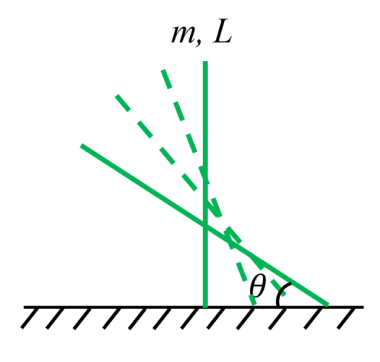
\includegraphics[width=\linewidth]{chapter3_rotating_rod_1}\\
			Figure 1
		\end{minipage}
		\quad
		\begin{minipage}{0.45\textwidth}
			\centering
			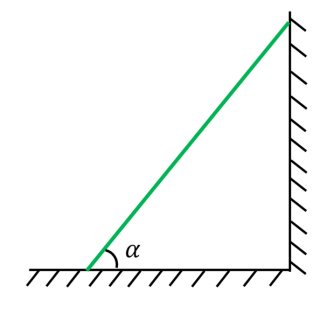
\includegraphics[width=\linewidth]{chapter3_rotating_rod_2}\\
			Figure 2
		\end{minipage}
	\end{center}
	(a) Calculate the angular velocity of the rod, when it has an angle of $\theta$ with respect to the ground
	as illustrated in Figure 1.\\
	(b) What is the final angular velocity $\omega_1$ of the rod before it hits the ground?\\
	(c) If the same rod is leaning to a frictionless wall with an initial angle of α to the frictionless
	ground (see Figure 2), what is the final angular velocity $\omega_2$ of the rod before it hits the ground?\\
	{\em Note that there is a possibility that the right end of the rod leaves from the wall before the rod hits the ground.}
\end{example}